\documentclass[12pt,a4paper]{article}
\usepackage[utf8]{inputenc}
\usepackage{amsmath}
\usepackage{amsfonts}
\usepackage{amssymb}
\usepackage{graphicx}
\usepackage[margin=0.5in]{geometry}

\graphicspath{{./images/}}
\author{Oleg Loshkin}
\title{\textbf{CSC}\\Convertible Scene Creator\\\textbf{Technical Document}}

\begin{document}

\maketitle
\section{Introduction}
	\begin{itemize}
		\item \textbf{Project's Context}
		\\As part of the game programming cursus at SAE Institute Geneva, for the \textbf{technical module GPR5100.2}, students of the second year must \textbf{assist students from the third year in completing their bachelor’s project.}\\\\
		This year, the third year's \textbf{PokFamily team} develops a \textbf{video game for the Switch} and PC using a tailored \textbf{in-house engine}.\\Second year students must \textbf{assist them} by creating various \textbf{tools they will need} in order to create their game.\\\\
		This document describes the functioning of the \textbf{Convertible Scene Creator} tool, \textbf{CSC} for short.
		
		\item \textbf{Project's Goals}
			\begin{itemize}
				\item Create a useful tool that the PokFamily team will use to create their video game.
				
				\item Learn to work in a non-academic environment in a team that depends on the student’s performance.
				
			\end{itemize}
			
		\item \textbf{Specific Problem}
		\\The PokFamily team uses the \textbf{Unity engine as an external editor}. The PokFamily team needs a tool to \textbf{export Unity scenes and prefabs} that may then be used inside the PokEngine.
	\end{itemize}
\newpage

\section{Requirements}
This project’s requirements have two origins:
\begin{itemize}
	\item \textbf{Academic requirements}
		\begin{itemize}
			\item The task given by the team has been understood and done in time.
			
			\item The tool is maintained by the student after the tool's completion.
			
			\item The tool must be user-friendly.
			
			\item The student understands how to manage data.
			
			\item The student understands how a game engine interfaces with a game engine editor.
			
			\item The student has organized himself and his work in a way to facilitate the work of others.
			
			\item The tool’s performance is reasonable.
			
			\item The implementation is appropriately sophisticated.
			
			\item The student understands the implications of non-academic teamwork.
			
		\end{itemize}
	\item \textbf{Pragmatic requirements}
		\begin{itemize}
			\item Convert Unity scene and prefab files to files readable by the PokEngine's parser via UPDC.
			
			\item The user must be able to interact with the tool via Unity.
			
			\item The code must satisfy the quality and style expected by the team. C++ coding style is defined in the Coding Style Document. C\# coding style is defined in UnityWorkOrganization document.
			
			\item The student must communicate with the team appropriately and be dependable.
			
	\end{itemize}
\end{itemize}

\section{Technologies Used}
\begin{itemize}
	\item \textbf{PokEngine}\\
		The \textbf{PokEngine} is the game engine developed by the PokFamily team. The engine is \textbf{written with C++ standard 2014} and \textbf{partly C++ standard 2014} for code running on the Nintendo Switch.\\
The engine has a parser that is capable of reading JSON files. This parser is used to import data exported from Unity with UPDC.

	\item \textbf{Unity 2019.1.10f}\\
		Unity 2019.1.10f is used as an \textbf{external editor}.
	
	\item \textbf{Visual Studio 2017}\\
		Visual Studio 2017 is used for development of the PokEngine.
	
	\item \textbf{Git}\\
		\textbf{github.com} is used for versioning for the \textbf{PokEngine source code}. \textbf{gitlab.com} is used for versioning for the \textbf{Unity prototype source code}. Git bash is used for most interactions with the git framework. Merge conflicts are solved manually via text editor and git bash.		
\end{itemize}
\newpage

\section{UML Diagram}
TODO

\section{Interaction with Overall Project}
\begin{center}
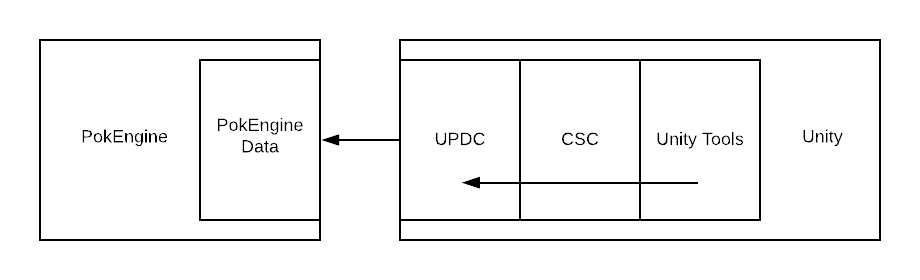
\includegraphics[scale=0.5]{CSCLocation}
\end{center}
\textbf{CSC integrates with UPDC to export scenes and prefabs}. As such, it interacts with Unity's database from which it creates .asset files for UPDC to export.

\section{Folder Hierarchy}
\begin{center}
\includegraphics[scale=0.425]{folderUPDC}
\end{center}

\section{Tackling Genericity}
In an \textbf{earlier version} of the tool, it \textbf{was capable of successfully exporting scenes} with their game objects, colliders, models and prefabs. \textbf{However, the implementation exportation of any additional components} located on game objects \textbf{would have required the user to dive deep into the code} of the CSC.\\\\
This is why the \textbf{tool was redesigned to allow easier implementation of exportation of new convertible components}. This was done by \textbf{splitting the ConvertibleSceneCreator between two .cs files} (ConvertibleSceneCreator.cs and Components.cs) using the "partial" keyword of the C\# language.\\\\ In doing so, \textbf{only the relevant part of CSC code is exposed to the user and the exportation implementation} for new convertible components \textbf{can be done by adding a few lines of code only} inside the ConvertibleSceneCreator class \textbf{at locations very explicitly commented}. The \textbf{user no longer needs to understand the functioning of CSC} in depth \textbf{to expand the tool}'s functionalities.\\\\
The decoupling of the tool in this manner did not require the need for runtime reflection, which can be tricky to implement. All that was needed were a few abstract classes and the use of some C\# generics.

\section{Tackling Polymorphism}
TODO: WIP second parser to remove empty fields TODO: update UPDC doc when done

\section{Exporting Prefabs}
TODO: prefab => fbx

\section{Exporting FBX and OBJ Files}
TODO WIP

\section{Integrating with ProBuilder}
TODO: WIP probuilder => prefab => fbx

\section{Potential Improvements}
\begin{itemize}
\item The prefab exportation had been done in a rush, the current implementation has a lot of room for improvement:
\begin{itemize}
\item WIP: There are way too many data structures defined to separate between different types of prefab objects, there must be a more elegant way to represent them.
\end{itemize}
\item While exportation of ProBuilder meshes is functional, it is implemented in a way as to duplicate already existing meshes. This is a behaviour that could be improved.
\item WIP: As a consequence of UPDC's implementation, polymorphism is not handled. A redesign of UPDC might make the implementation of collider exportation more elegant.
\end{itemize}

\section{Summary}
TODO

\end{document}
